\documentclass{beamer}

%%%%%%%%%%%%%%%%%%%%%%%%%%%%%%%%%%%%%%%%%%%%%%%%%%%%%%%%%%%%%%%%
%%%                  Themes and such                         %%%
%%%%%%%%%%%%%%%%%%%%%%%%%%%%%%%%%%%%%%%%%%%%%%%%%%%%%%%%%%%%%%%%
\mode<presentation>
{
  %\usetheme{Copenhagen}  
  \usetheme{Warsaw}  
  %\usetheme{Malmoe}  
   % \setbeamertemplate{headline}{}
  %make my huge toc fit on one slide (and not look horrible)
  %\setbeamerfont{subsection in toc}{series=\bfseries}
  \setbeamerfont{subsection in toc}{size=\tiny,series=\bfseries}
}

%%%%%%%%%%%%%%%%%%%%%%%%%%%%%%%%%%%%%%%%%%%%%%%%%%%%%%%%%%%%%%%%
%%%                       Packages                           %%%
%%%%%%%%%%%%%%%%%%%%%%%%%%%%%%%%%%%%%%%%%%%%%%%%%%%%%%%%%%%%%%%%
\usepackage{multimedia}
\usepackage{multirow}
\usepackage{subfigure}
\usepackage{amsmath}
\usepackage{parskip}
\setlength{\parskip}{\smallskipamount} 
\usepackage{color}
\usepackage{tikz}
%\usepackage{tcolorbox}

% Define commands
 \newcommand{\half}{\ensuremath{\frac{1}{2}}}

 \newcommand{\bea}{\begin{eqnarray}}
 \newcommand{\eea}{\end{eqnarray}}
 \newcommand{\beq}{\begin{equation}}
 \newcommand{\eeq}{\end{equation}}
 \newcommand{\bed}{\begin{displaymath}}
 \newcommand{\eed}{\end{displaymath}}

 \newcommand{\pd}[2]{\dfrac{\partial #1}{\partial #2}}
 \newcommand{\pf}[2]{\dfrac{d #1}{d #2}}
 \newcommand{\pdt}[2]{\dfrac{\partial^2 #1}{\partial #2^2}}
 \newcommand{\pft}[2]{\dfrac{d^2 #1}{d #2^2}}
 \newcommand{\pdtno}[2]{\dfrac{\partial^2 #1}{\partial #2}}
 \newcommand{\pdd}[3]{\dfrac{\partial^2 #1}{\partial #2 \partial #3}}
 \newcommand{\pff}[3]{\dfrac{d^2 #1}{d #2 d #3}}

 \graphicspath{{../figures/}}

\makeatletter
\newenvironment{noheadline}{
    \setbeamertemplate{headline}{}
    \addtobeamertemplate{frametitle}{\vspace*{-1.5\baselineskip}}{}
}{}
\makeatother

%%%%%%%%%%%%%%%%%%%%%%%%%%%%%%%%%%%%%%%%%%%%%%%%%%%%%%%%%%%%%%%%
%%%                     Title Info                           %%%
%%%%%%%%%%%%%%%%%%%%%%%%%%%%%%%%%%%%%%%%%%%%%%%%%%%%%%%%%%%%%%%%

\title[Time Dependent Discrete Adjoint]
{
Adjoint-Based Derivative Evaluation Methods for Flexible Multibody Systems
}

\author[K. Boopathy and G. J. Kennedy - SMDO Laboratory]
{
  \Large {Komahan Boopathy} \\ 
  and \\
  \Large {Dr. Graeme J. Kennedy} \\
}

\institute[GeorgiaTech]
{
  \large Structures and Multidisciplinary Optimization Laboratory \\
  ~\\
  School of Aerospace Engineering\\
  Georgia Institute of Technology\\
 Atlanta, GA
}

\logo{%
 %   \makebox[0.95\paperwidth]{%
  
\includegraphics[width=2cm,keepaspectratio]{ae-logo.png}
  %\hfill
  %
\includegraphics[width=2cm,keepaspectratio]{ae-logo.png}
  %}
}

\date[\today]
{
\small \today
}

\begin{document}

%\setbeamertemplate{background}{
%  \begin{tikzpicture}
%    \node[opacity=.01,inner sep=0pt]{
%     
\includegraphics [height=\paperheight]{gt.png}};
%  \end{tikzpicture}
%}

% Now we install the new template for the following frames:
%\usebackgroundtemplate{%
%  \includegraphics[width=\paperwidth,height=\paperheight]{}}

\begin{frame}
  \titlepage
\end{frame}

%\setbeamertemplate{background}{
%  \begin{tikzpicture}
%    \node[opacity=.003,inner sep=0pt]{
%     
\includegraphics [height=\paperheight]{gt.png}};
%  \end{tikzpicture}
%}
%\begin{frame}
%  \frametitle{Outline}
%  \tableofcontents
%\end{frame}

%\addtobeamertemplate{frametitle}{}{%
%  \begin{tikzpicture}[remember picture, overlay]
%    \node[anchor=north east, xshift=4.5pt, yshift=7.5pt] at (current page.north east)
%         {
\includegraphics[height=0.8cm]{ae-logo.png}};
%  \end{tikzpicture}
%}

\begin{frame}[shrink]\frametitle{Motivation: Need for Derivatives}\scriptsize{
    \begin{minipage}{\linewidth}
      \begin{minipage}{0.5\linewidth}
        \begin{block}{Finite differences and complex-step}   
          \begin{itemize}
          \item Simple, robust but \alert{inefficient}
          \item Doesn't require knowledge of governing equations
          \end{itemize}
        \end{block}
        \begin{block}{Adjoint and direct method}
          \begin{itemize}
          \item Efficient, robust but complicated
          \item Precise to the tolerance to which the governing ODEs/DAEs/PDEs
            are solved $(10^{-8}, 10^{-12}, 10^{-16})$
          \item Direct -- efficient for \alert{\# functions}
          \item Adjoint -- efficient for \alert{\# variables}
          \item Requires knowledge of governing equations (semi-analytic)
            \begin{itemize}
            \item Calculus
            \item Linear algebra
            \item Graph theory {$+$}
            \end{itemize}
          \item Adjoint details, to follow...
          \end{itemize}
        \end{block}
      \end{minipage}
      \begin{minipage}{0.5\linewidth}
        \hfill
        \begin{tikzpicture}
          \node {
            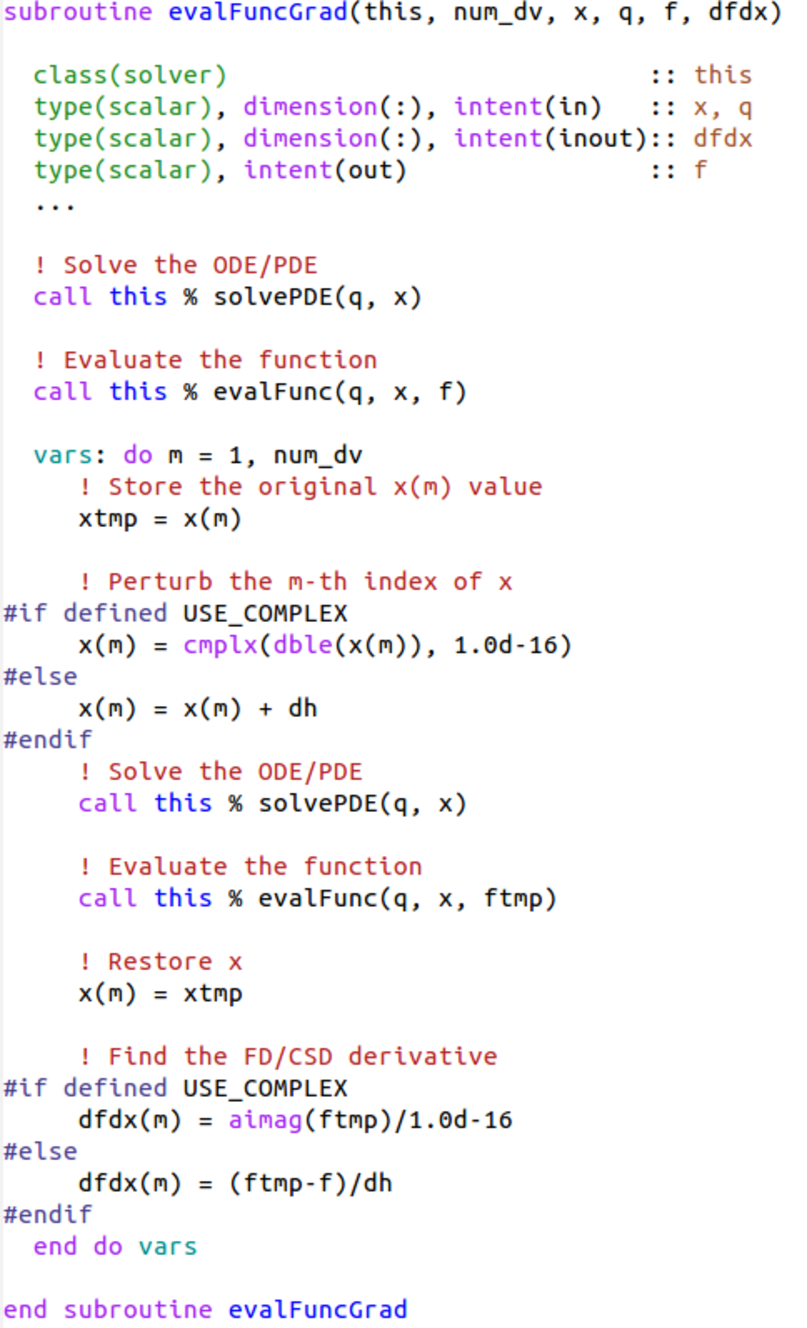
\includegraphics[height=0.8\paperheight]{fd-csd.pdf}
          };
        \end{tikzpicture}
      \end{minipage}
    \end{minipage}
  }
\end{frame}

%\begin{noheadline}
\begin{frame} \frametitle{Background}
  \tiny{
  \begin{block}{101. Notation:}
    \begin{tabbing}
      XXXXXX \= xxxx\kill
      $t$     \> time \\
      $k$     \> time index \\
      $x$     \> design variables \\
      $m$     \> number of design variables \\
      $u,v,w$ \> state variables \\
      $n$  \> number of state variables \\
      $R, S, T$ \> governing (constraint) equations  \\
      $\lambda,\psi,\phi$ \> adjoint variables  \\
      $F$     \> objective function \\
      $\cal{L}$ \> Lagrangian \\
    \end{tabbing}
  \end{block}
  \begin{center}
    \begin{block}{1. Objective Function:}
      A time-averaged objective function is considered (e.g. mean lift,
      mean potential energy, mean thermal-stress). We can approximate
      the integral as a discrete sum:
      \begin{equation}\label{eqn:time-averaged-function}
        F = \frac{1}{T}\int_{0}^T f_k(u,v,w,x,t)~dt=\sum_{k=0}^N h f_k(u_k,v_k,w_k,x)
      \end{equation}
      Other possibilities for the choice of objective function exist
      too.
    \end{block}
  \end{center}
  }
\end{frame}

\begin{frame}[shrink] \frametitle{Background}
    \tiny{
  \begin{center}

%  \begin{columns}
%    \column{0.5\textwidth}
%    \column{0.5\textwidth}
%  \end{columns}


  \begin{block}{3. Lagrangian:}
    It would be nice and handy to pack all separate equations (objects)
    into one equation (object) to operate with. We introduce
    \textcolor{red}{$\lambda_k$}, \textcolor{orange}{$\psi_k$} and
    \textcolor{blue}{$\phi_k$} as the adjoint variables associated with
    each of these function objects at the each time step and the
    Lagrangian function is written as:
    \begin{equation}\label{eqn:nbg-lagrangian}
      {\cal{L}} = \textcolor{brown}{\sum_{k=0}^N h f_k} + \textcolor{red}{ \sum_{k=0}^N h \lambda_k^T R_k} 
      +  \textcolor{orange}{ \sum_{k=0}^N\psi_k^T S_k} +  \textcolor{blue}{ \sum_{k=0}^N\phi_k^T T_k}.
    \end{equation}
  \end{block}
  \begin{block}{Remark}
    The Lagrangian is a linear ``\texttt{\underline{F}AXPY}'' 
    operator  (why not!) operating on vector objects -- just like \texttt{\underline{S}AXPY}, 
    \texttt{\underline{D}AXPY}, \texttt{\underline{Z}AXPY} (being Fortranic).
    Here $\lambda,~\phi,~\psi$ adjoint variables: they
    manifest themselves as simple-scaling-scalars in linear-algebra and
    as Lagrange multipliers in the context of optimization.
  \end{block}
  \begin{block}{Remark}
    When decoupling is possible one or more of the
    constraint equations fold into other equations and therefore the
    corresponging adjoint variable need not be included in the
    formulation of the Lagrangian, but is typically done for the sake of
    convenience/generality of the implementation.
  \end{block}
  \end{center}
  }
\end{frame}

\begin{frame}\frametitle{Background}\tiny{

    \begin{minipage}{\linewidth}
      \begin{minipage}{0.49\linewidth}
        \begin{block}{4. Solution:}
          For each timestep $k$:
          \begin{block}{Forward Mode}
            \begin{itemize}
            \item Find state variables $\mathbf{u}_K$
            \item Newton's method based on linearization of governing equations:
              {$ \pd{\mathbf{R}_k^p}{\mathbf{u}_k^p} \Delta \mathbf{u}_k^p   = - R_k$; $\mathbf{u}_k^p = \mathbf{u}_k^p + \Delta \mathbf{u}_k^p$} 
            \item Involves $p$ linear solutions
            \end{itemize}
          \end{block}
          \begin{block}{Reverse Mode}
            \begin{itemize}
            \item Find adjoint variables: $\lambda$, $\psi$ and
              $\phi$ and 
              and total derivative $\pf{f}{x}$
            \item $1/p$ of computational time \alert{per function}
            \item Linear problem of solving stationary points of the
              Lagrangian w.r.t. the states:
              {${\pd{\cal{L}}{u_k}},{\pd{\cal{L}}{v_k}},
                {\pd{\cal{L}}{w_k}} = 0$}
            \end{itemize}
          \end{block}
        \end{block}
      \end{minipage}
      \begin{minipage}{0.49\linewidth}
%        \hfill
%        \begin{tikzpicture}
%          \node[above]{
%            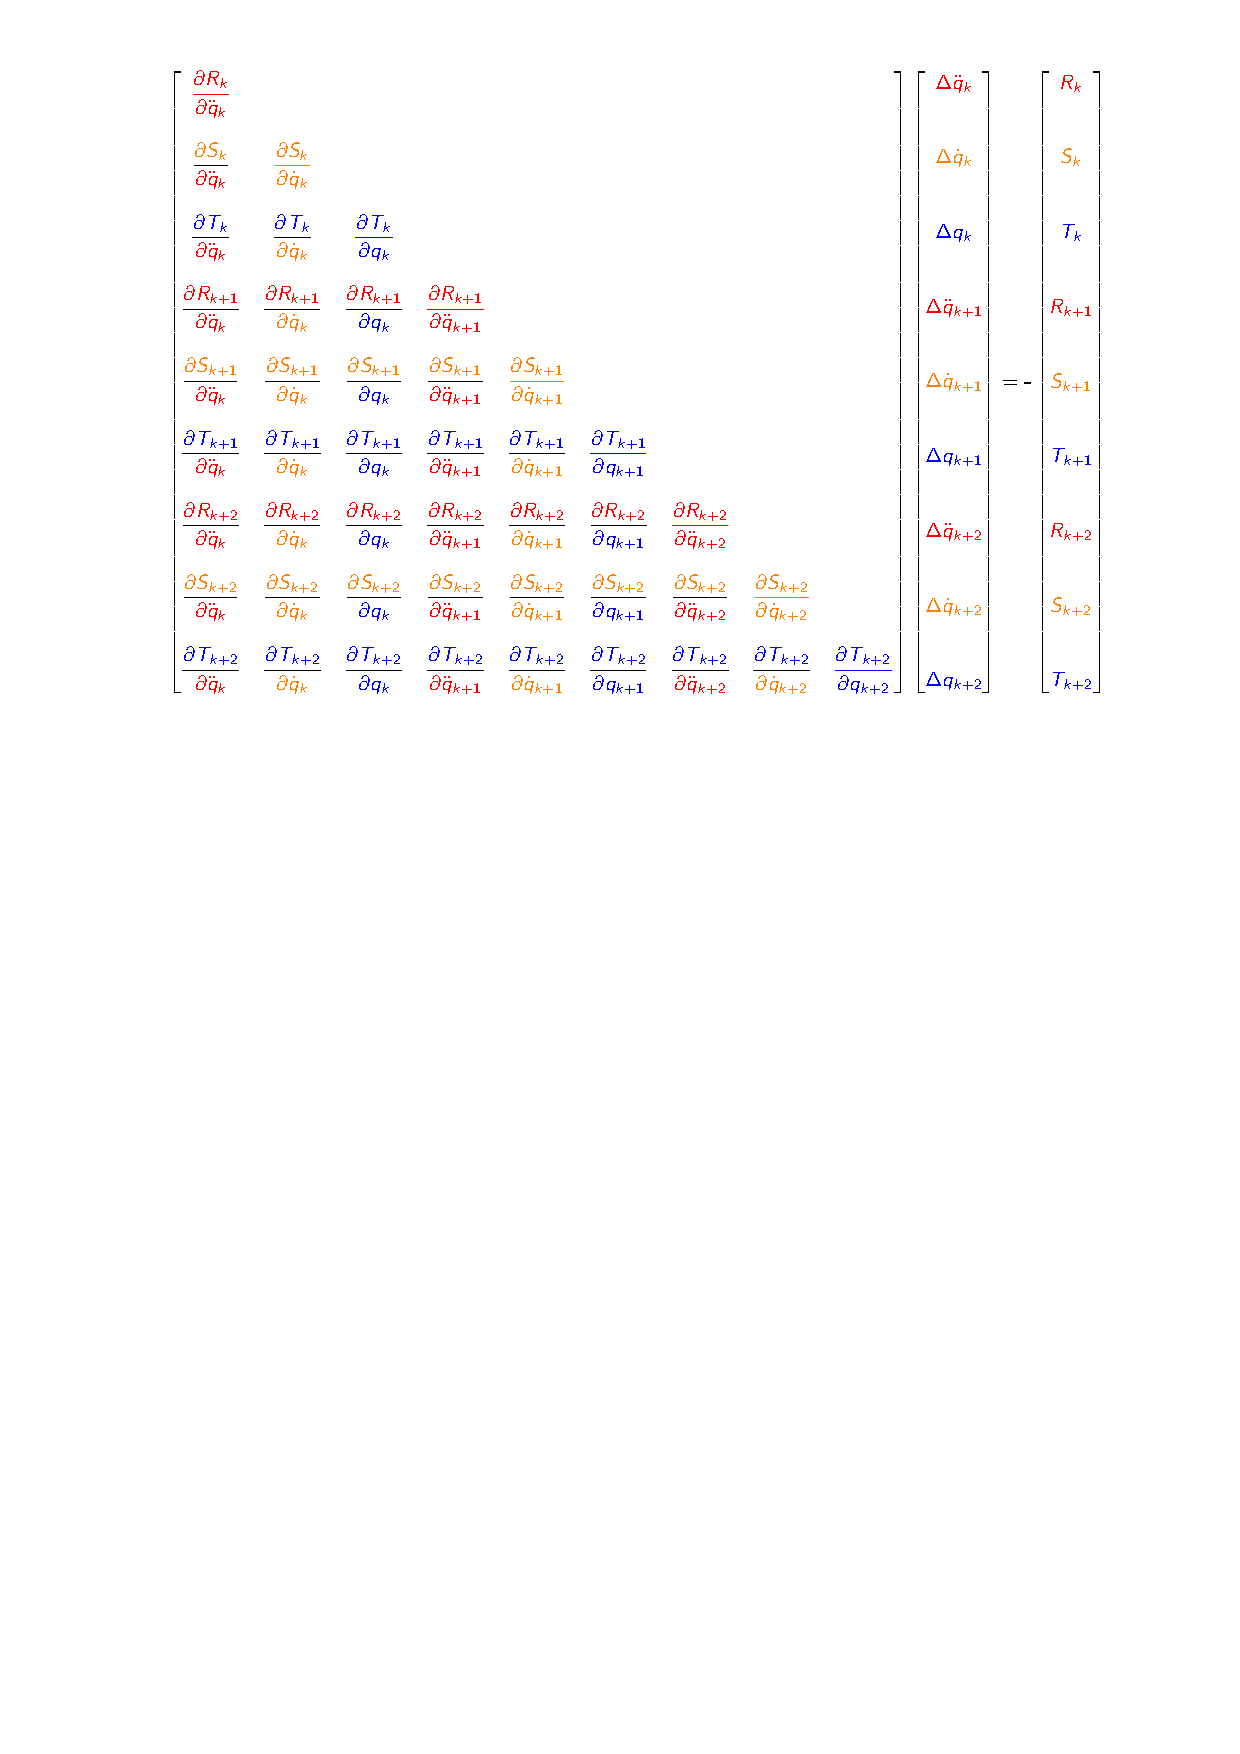
\includegraphics[height=0.49\textwidth]{general-forward-matrix.pdf}
%          };
%          \node[below]{
%            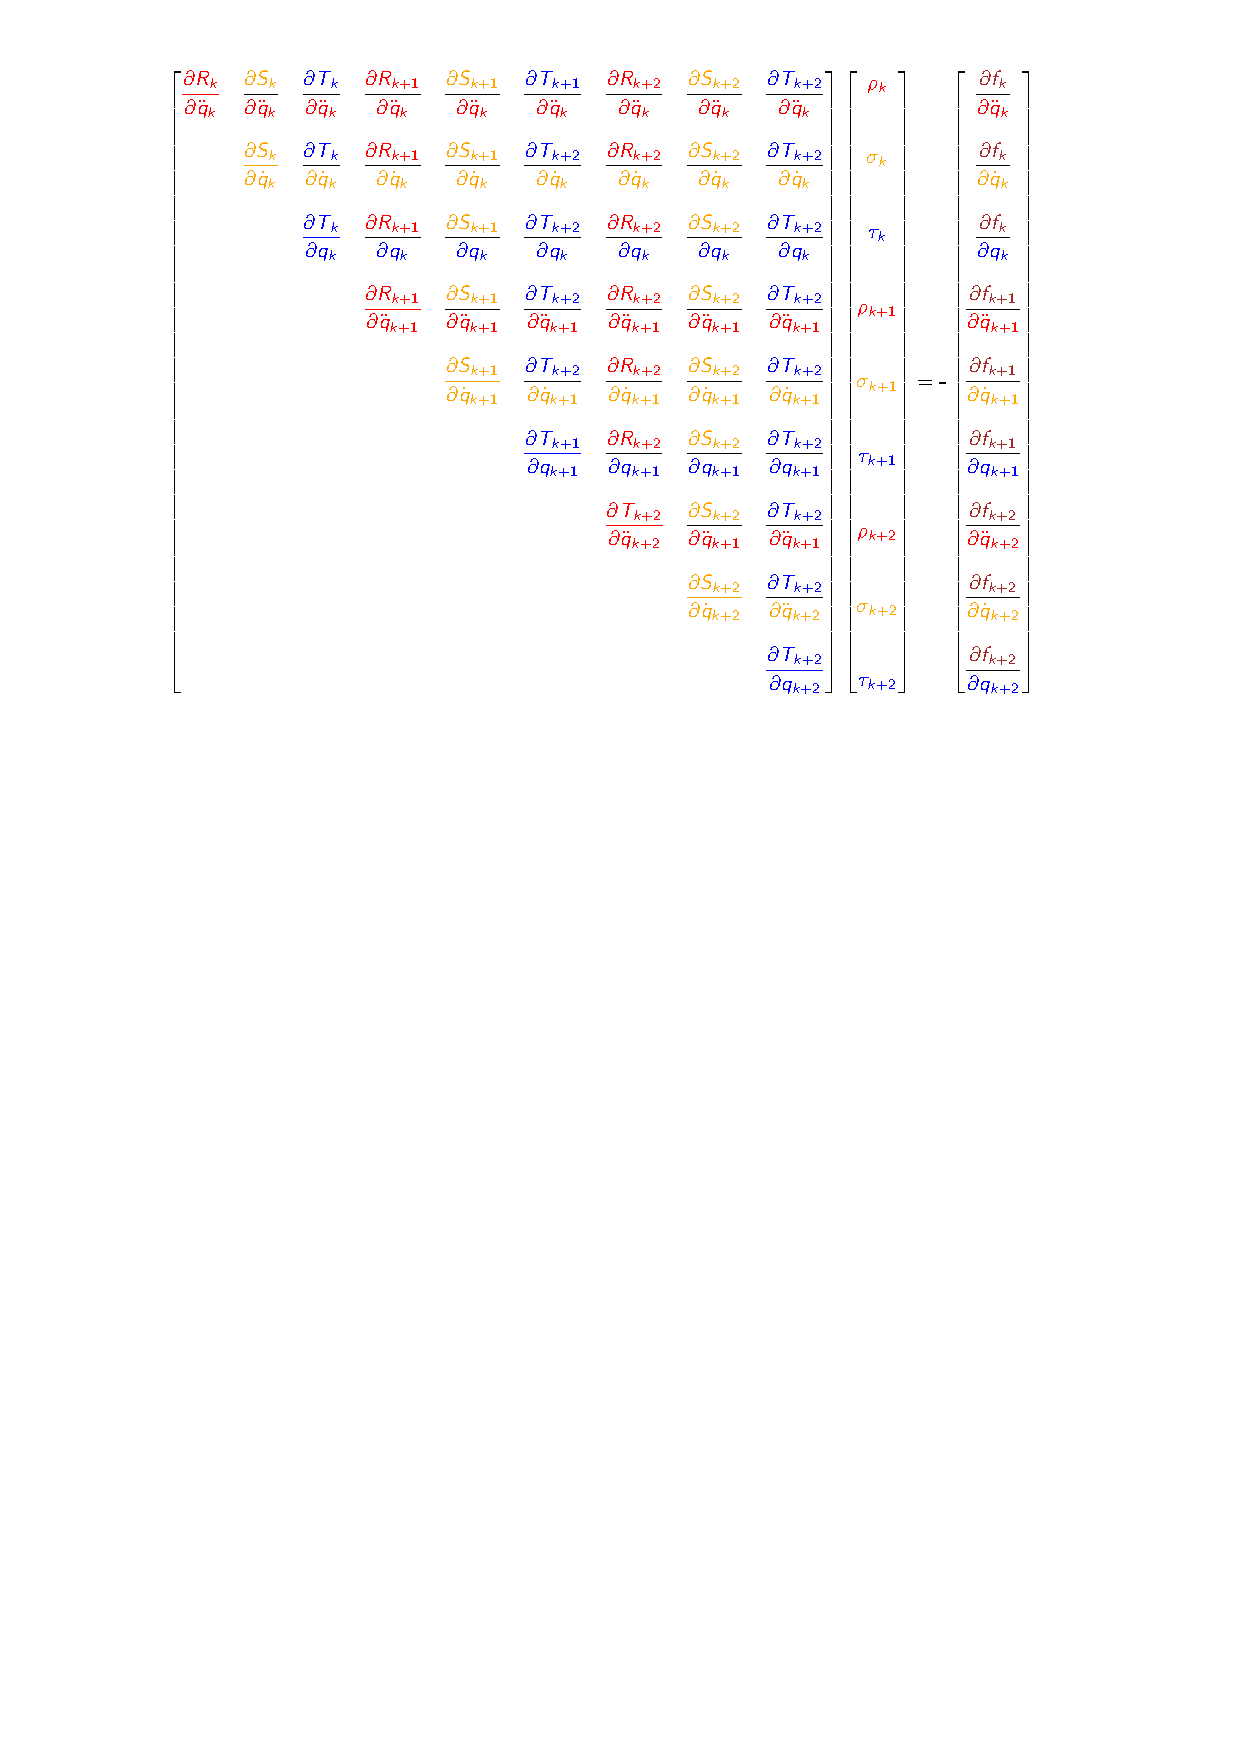
\includegraphics[height=0.49\textwidth]{general-reverse-matrix.pdf}
%          };
%        \end{tikzpicture}       
        \begin{figure}
          \centering
          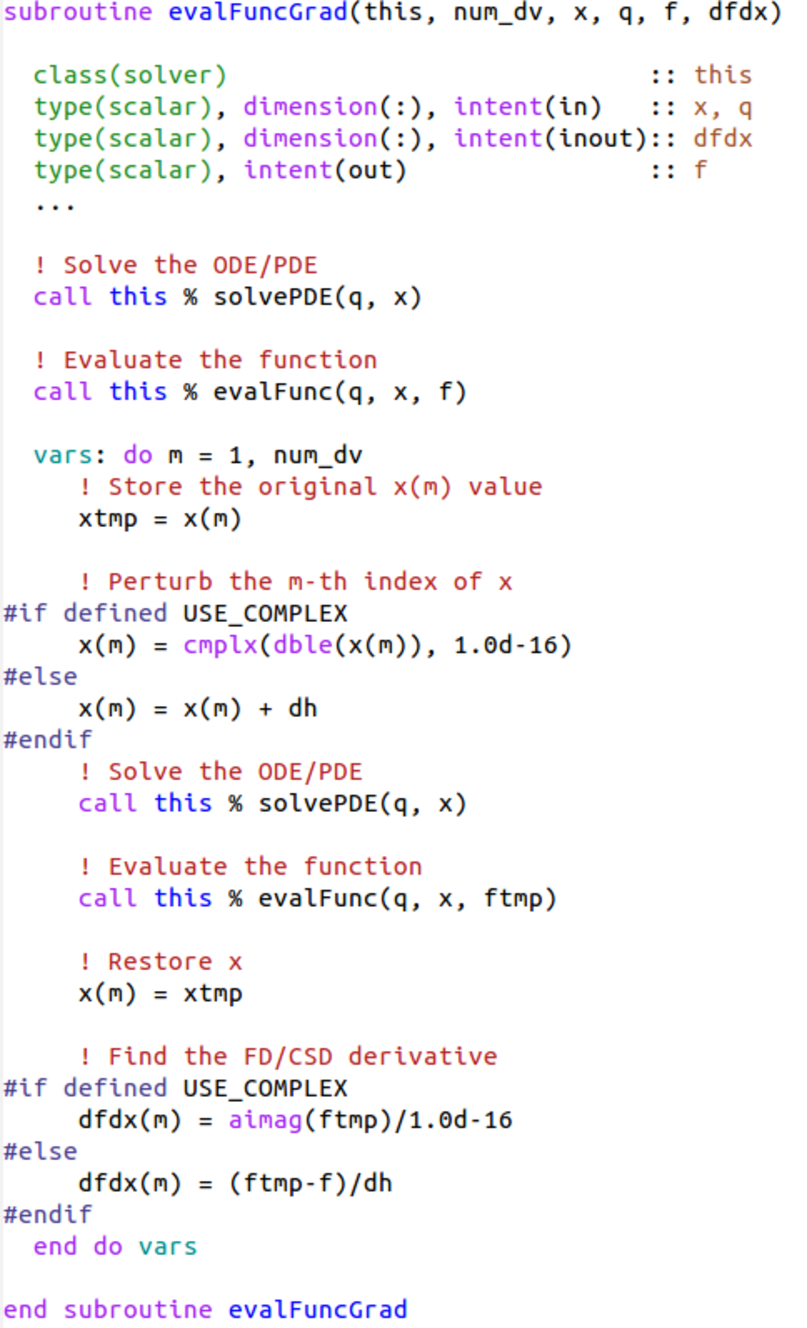
\includegraphics[trim={2pt 0 0 0}, clip,width=0.75\textwidth]{fd-csd.pdf}
        \end{figure}
      \end{minipage}
    \end{minipage}
  }
\end{frame}

\begin{frame}\frametitle{Background}\scriptsize{

    \begin{block}{5. Total Derivative:}
      The total derivative can be
      written as a \underline{linear combination} of contributions from the function
      of interest and the constraints:
      \begin{equation}\label{eqn:nbg-total-derivative}
        \pd{\cal{L}}{x} = \pd{F}{x} = 
        \textcolor{brown}{\sum_{k=0}^N h \pd{f_k}{x}^T} + 
        \textcolor{red}{\sum_{k=0}^N h \pd{R_k}{x}^T \lambda_k} + 
        \textcolor{orange}{\sum_{k=0}^N \pd{S_k}{x}^T \psi_k} + 
        \textcolor{blue}{\sum_{k=0}^N \pd{T_k}{x}^T \phi_k}.
      \end{equation}
    \end{block}
    \begin{block}{Remark}
      The objective function value $F$ and the gradient $\pf{F}{x}$ goes
      to the optimization code.
    \end{block}
  }
\end{frame}

\begin{frame}\frametitle{Flexible Multibody Dynamics}\tiny{

    \begin{block}{Context of Structural Dynamics and Time Marching}
      \begin{minipage}{0.45\linewidth}
        \begin{tabbing}
          XXXXXX \= xxxx\kill
          $t$     \> time \\
          $k$     \> time index \\
          $x$     \> design variables \\
          $m$     \> number of design variables \\
          \colorbox{blue!20}{$u,v,w$} \> \colorbox{blue!20}{state variables} \\
          $n$  \> number of state variables \\
          \colorbox{green!20}{$R, S, T$} \> constraint governing equations  \\
          $\lambda ,~ \psi ,~\phi$ \> adjoint variables  \\
          $F$     \> objective function \\
          $\cal{L}$ \> Lagrangian \\
        \end{tabbing}
      \end{minipage}\hfill
      \begin{minipage}{0.45\linewidth}
        \begin{tabbing}
          XXXXXX \= xxxx\kill
          $t$     \> time \\
          $k$     \> time index \\
          $x$     \> design variables \\
          $m$     \> number of design variables \\
          \colorbox{blue!20}{$q,\dot{q},\ddot{q}$} \> \colorbox{blue!20}{position, velocity and acceleration states} \\
          $n$  \> number of state variables \\
          \colorbox{green!20}{$R, S, T$} \> constraint governing equations  \\
          $\lambda ,~ \psi ,~\phi$ \> adjoint variables  \\
          $F$     \> objective function \\
          $\cal{L}$ \> Lagrangian \\
        \end{tabbing}
      \end{minipage}
    \end{block}
    
  The residual of the governing equations from structural dynamics
  can be posed as: 
  \begin{equation}\label{eqn:nbg-residual}
    \textcolor{red}{R_k = R_k(\underline{\ddot{q}_k}, \dot{q}_k, q_k, x) = 0}.
  \end{equation}
  \begin{example} 
    $R = m\ddot{q} + c\dot{q} + k{q} = 0$, x = $[m,
      c, k]$ can be the design variables of choice, the objective be
    minimizing the time-averaged potential energy $F = \frac{1}{T}
    \int_{0}^T f_k~dt$, where $f_k = \frac{1}{2} kq^2$ is the
    instantaneous PE.
  \end{example}
  }
\end{frame}

\begin{frame}
  \frametitle{Further Directions}

  \begin{block}{Adjoint}
    
    \begin{itemize}
    \item AUTOMATIC evaluation of adjoint -- yes, we can!
      \begin{itemize}
      \item Based on \texttt{type(integrator)} -- leaverage smart
        data structures and modern constructs, graph theory
      \item NOT automatic differentiation (AD)!
      \end{itemize}
      
    \item Applications:
      
      \begin{enumerate}
      \item Optimization
      \item Error estimation
      \item Mesh refinement
      \item $\ldots$
      \end{enumerate}
      
    \end{itemize}
    
  \end{block}

  \begin{block}{Direct}
    Explore time dependent direct sensitivities
  \end{block}  
\end{frame}

\end{document}


\begin{frame}\frametitle{Matrix Structure}
  \begin{block}{Forward Mode}
    \begin{figure}
      \centering
      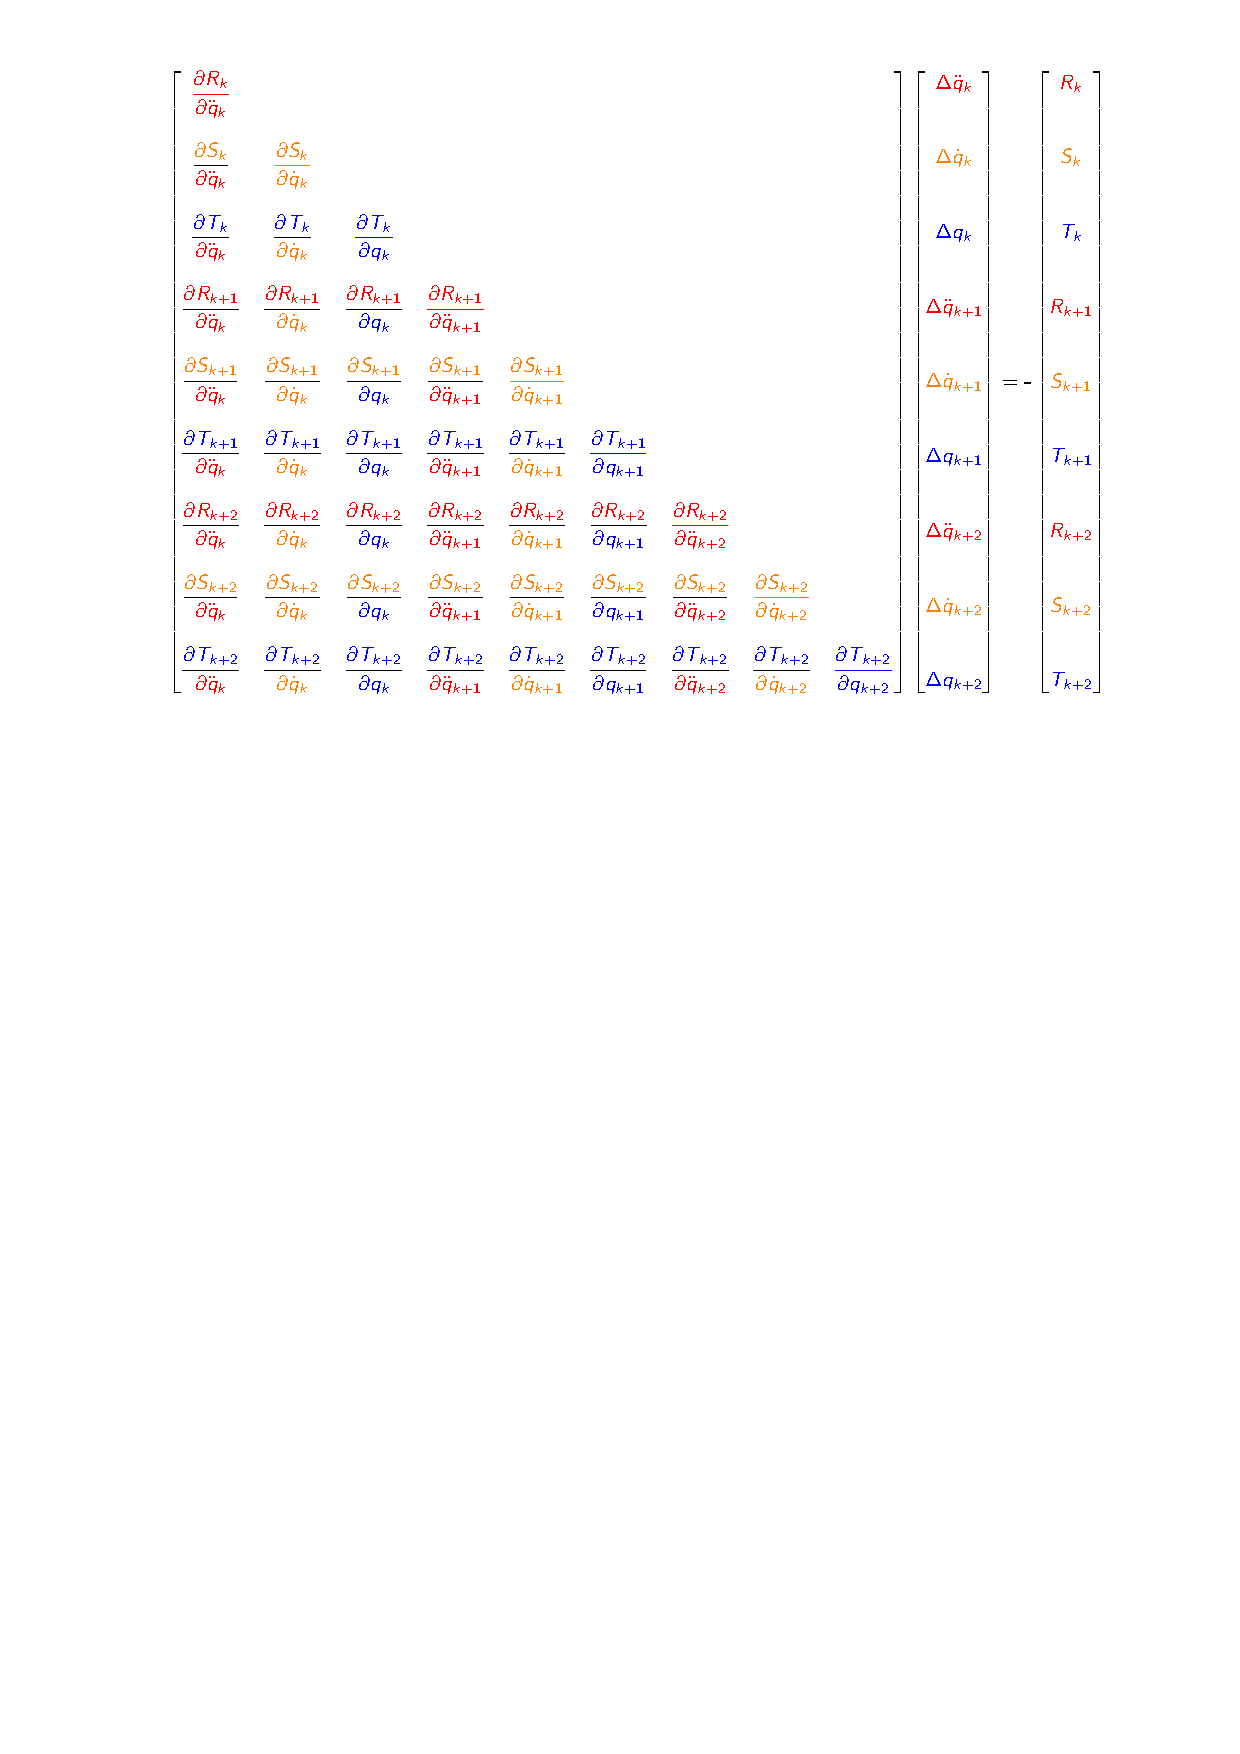
\includegraphics[width=\textwidth]{general-forward-matrix.pdf}
      \label{Forward Mode}
    \end{figure}
  \end{block}
\end{frame}
\begin{frame}\frametitle{Matrix Structure}
  \begin{block}{Reverse Mode}
    \begin{figure}
      \centering
      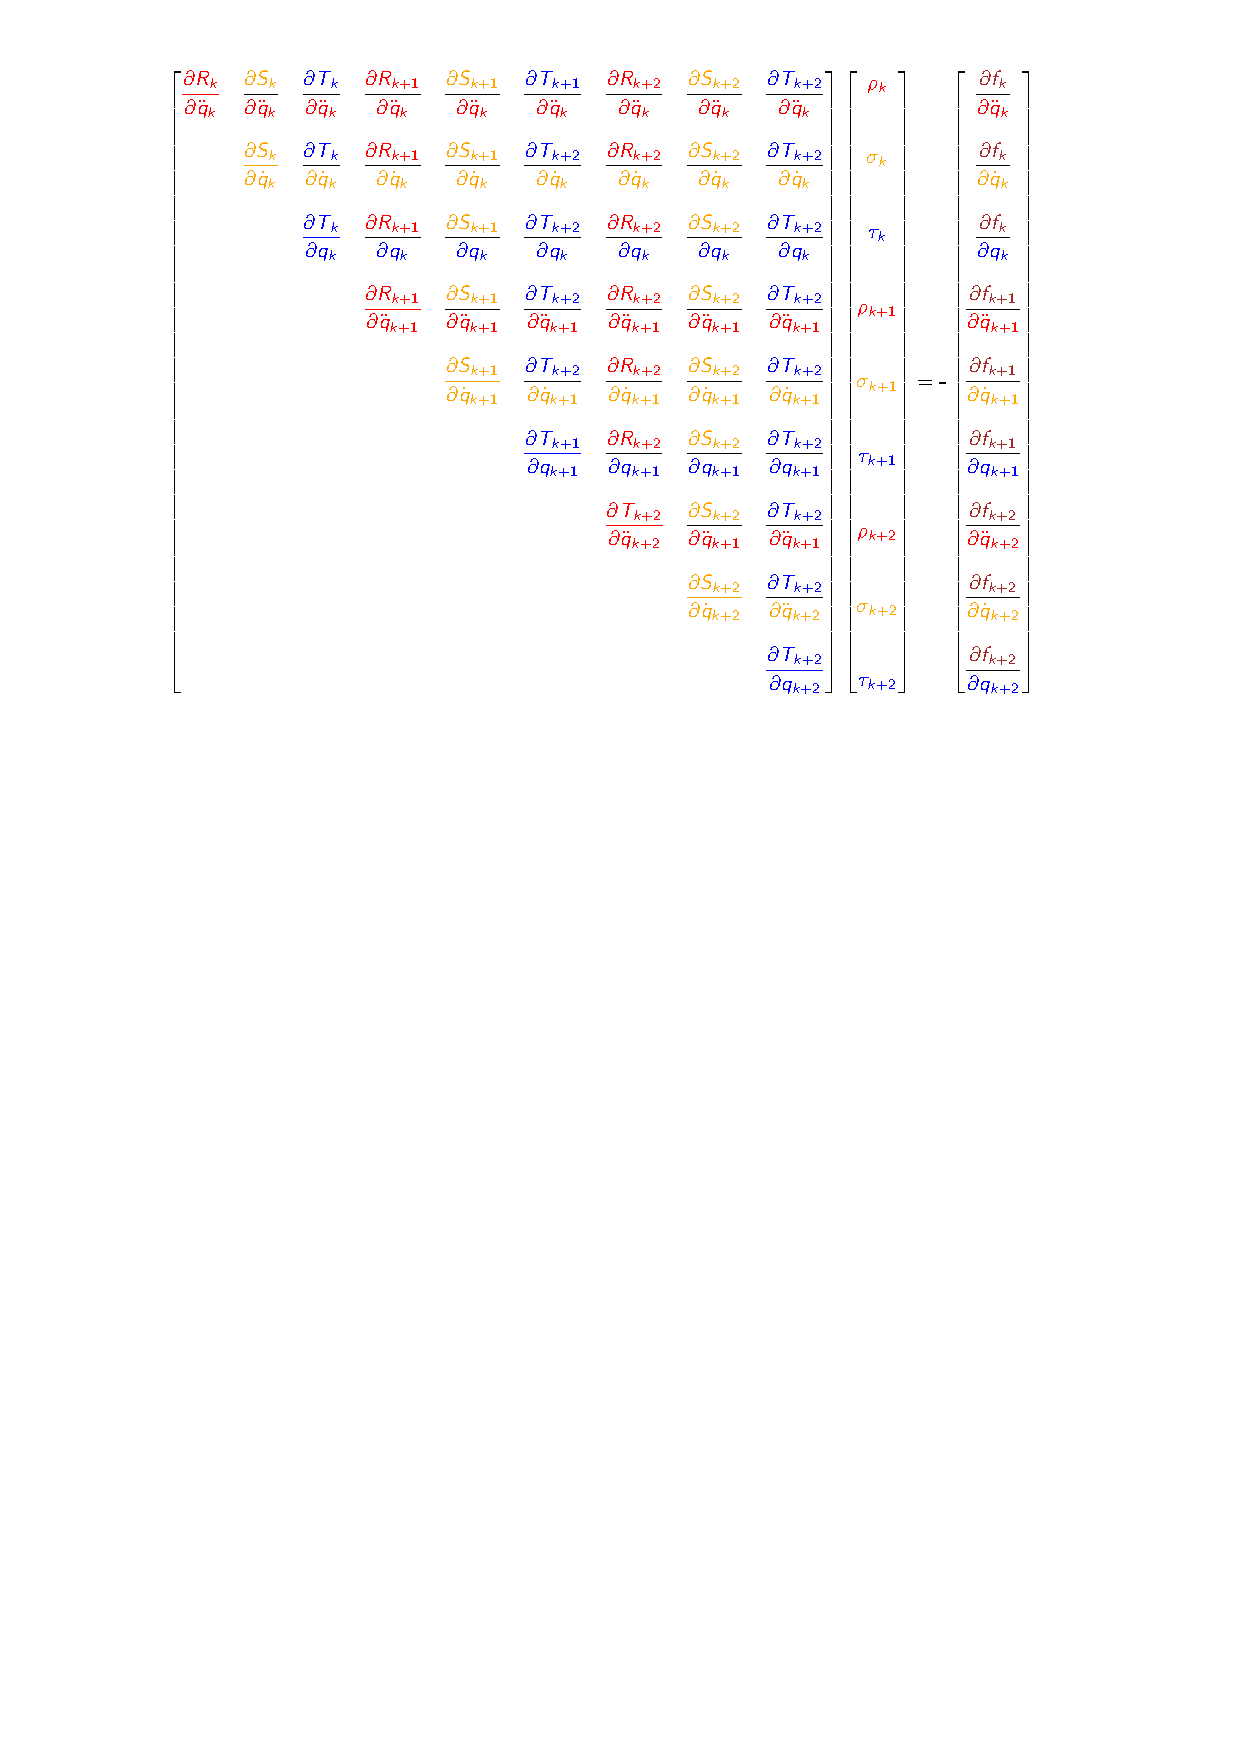
\includegraphics[width=0.925\textwidth]{general-reverse-matrix.pdf}
      \label{Reverse Mode}
    \end{figure}
  \end{block}  
\end{frame}

\begin{frame}[allowframebreaks,fragile]\frametitle{Newmark--Beta--Gamma Adjoint}
  \scriptsize{
    \begin{minipage}{0.6\linewidth}
      We use \textbf{Newmark--Beta--Gamma (NBG)} time-marching method to
      integrate and solve for the states over time.  The states
      approximation equations are:
      \begin{equation}\label{eqn:nbg-approx-qdot}
        \textcolor{orange}{S_k =  \dot{q}_{k-1}  + (1-\gamma) h \ddot{q}_{k-1} +  \gamma h \ddot{q}_{k}- \dot{q}_k=0, }
      \end{equation}
      \begin{equation}\label{eqn:nbg-approx-q}
        \textcolor{blue}{T_k = {q}_{k-1} + h \dot{q}_{k-1} +\frac{1-2\beta}{2}
          h^2\ddot{q}_{k-1} + \beta h^2 \ddot{q}_k-{q}_k=0}. 
      \end{equation}
      The underlined varibles are the primary variables in each equation.
      Eq~\eqref{eqn:nbg-residual} comes from the governing physics of
      the system. Eqs.~\eqref{eqn:nbg-approx-qdot} and
      ~\eqref{eqn:nbg-approx-q} come from the time-marching
      scheme. Therefore, the equations $S_k$ and $T_k$ are independent
      of the design variables $x$ -- they do not contribute to the total
      derivative. 
    \end{minipage}
    \begin{minipage}{0.39\linewidth}
      \begin{figure}
        \centering
        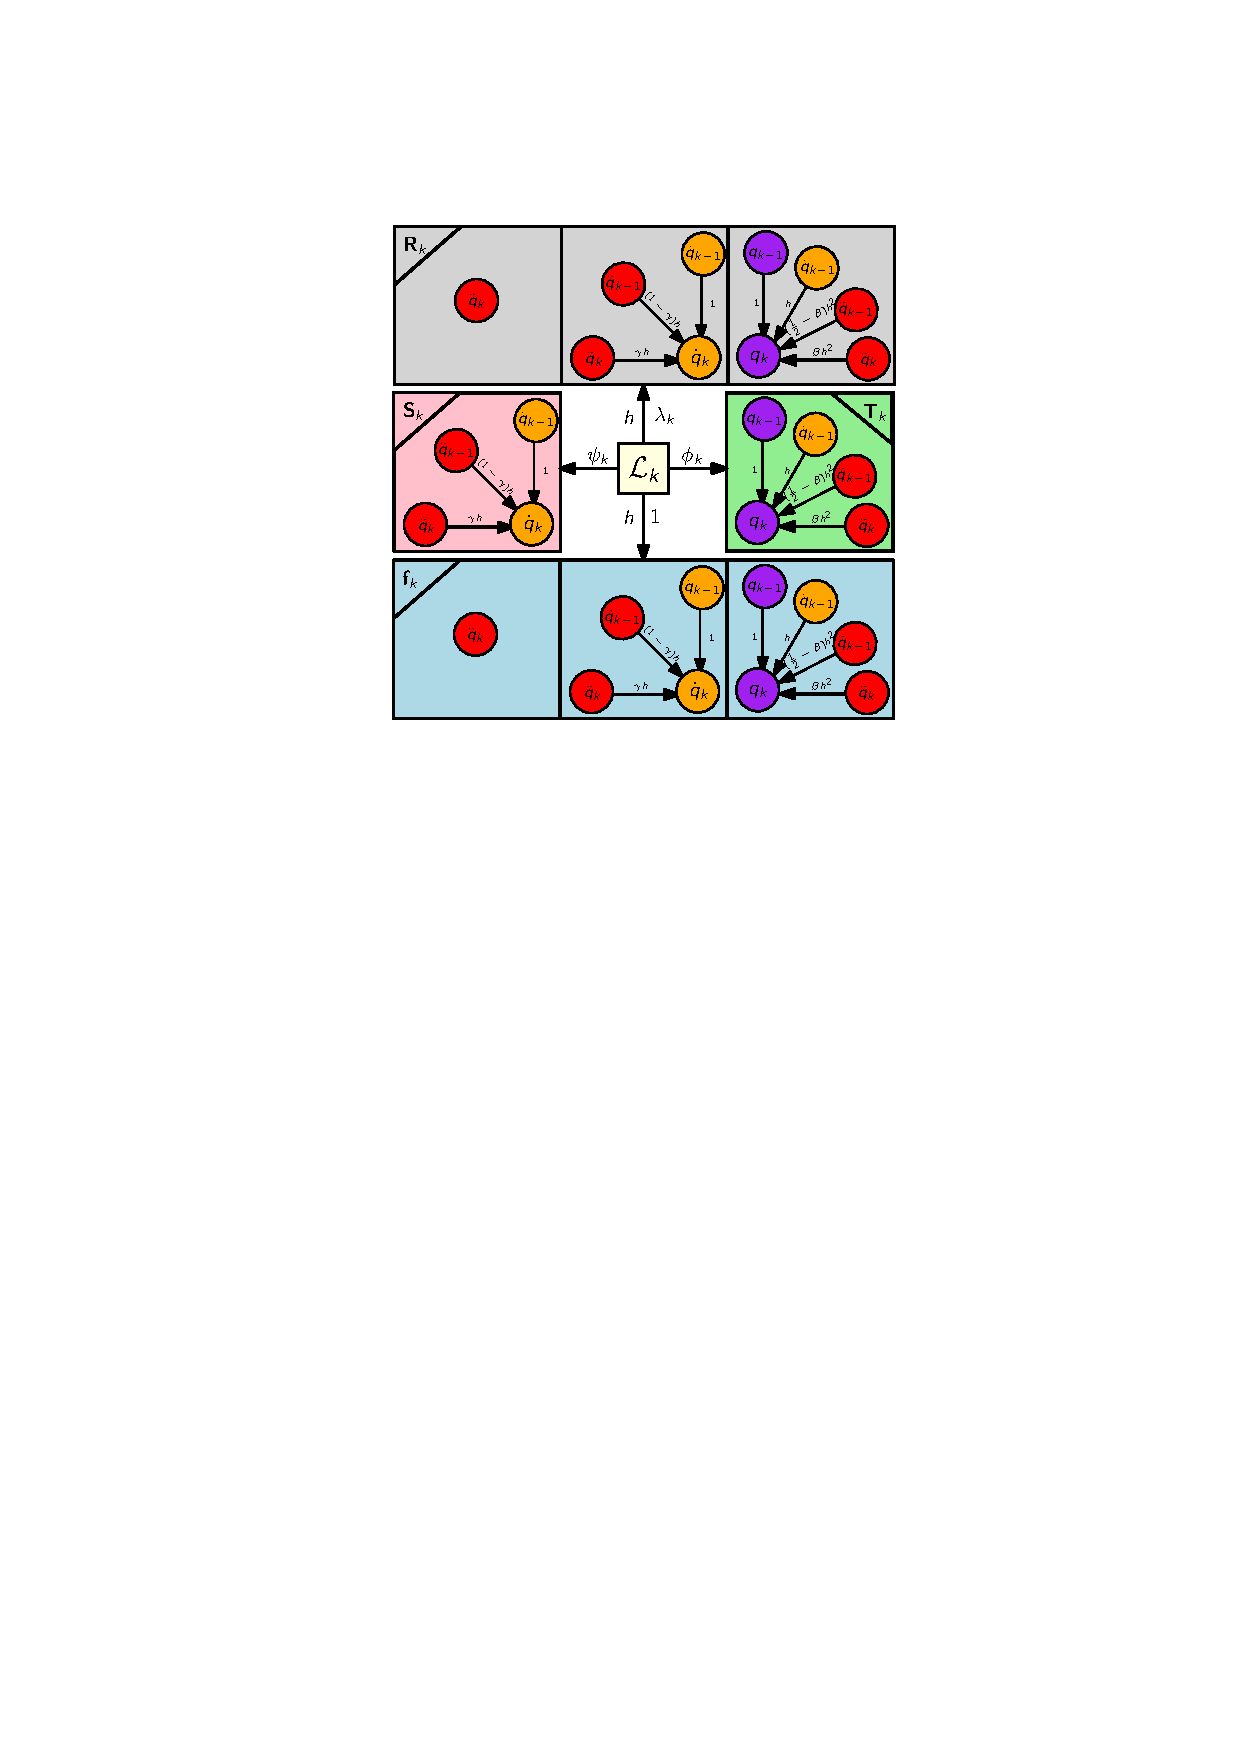
\includegraphics[width=\textwidth]{nbg-lagrangian.pdf}
        %\caption{Illustrations showing the working of NBG method.}
        \label{fig:nbg-illustration}
      \end{figure}
    \end{minipage}
    
    \textbf{Total Derivative:}
    \begin{equation}\label{eqn:nbg-total-derivative}
      \pd{\cal{L}}{x} = \pd{F}{x} = \textcolor{brown}{\sum_{k=0}^N h \pd{f_k}{x}^T} +\textcolor{red}{ \sum_{k=0}^N h
        \pd{R_k}{x}^T \lambda_k}.
    \end{equation}

  %    \begin{minipage}{1.0\linewidth}
  %      \begin{figure}
  %        \centering
  %        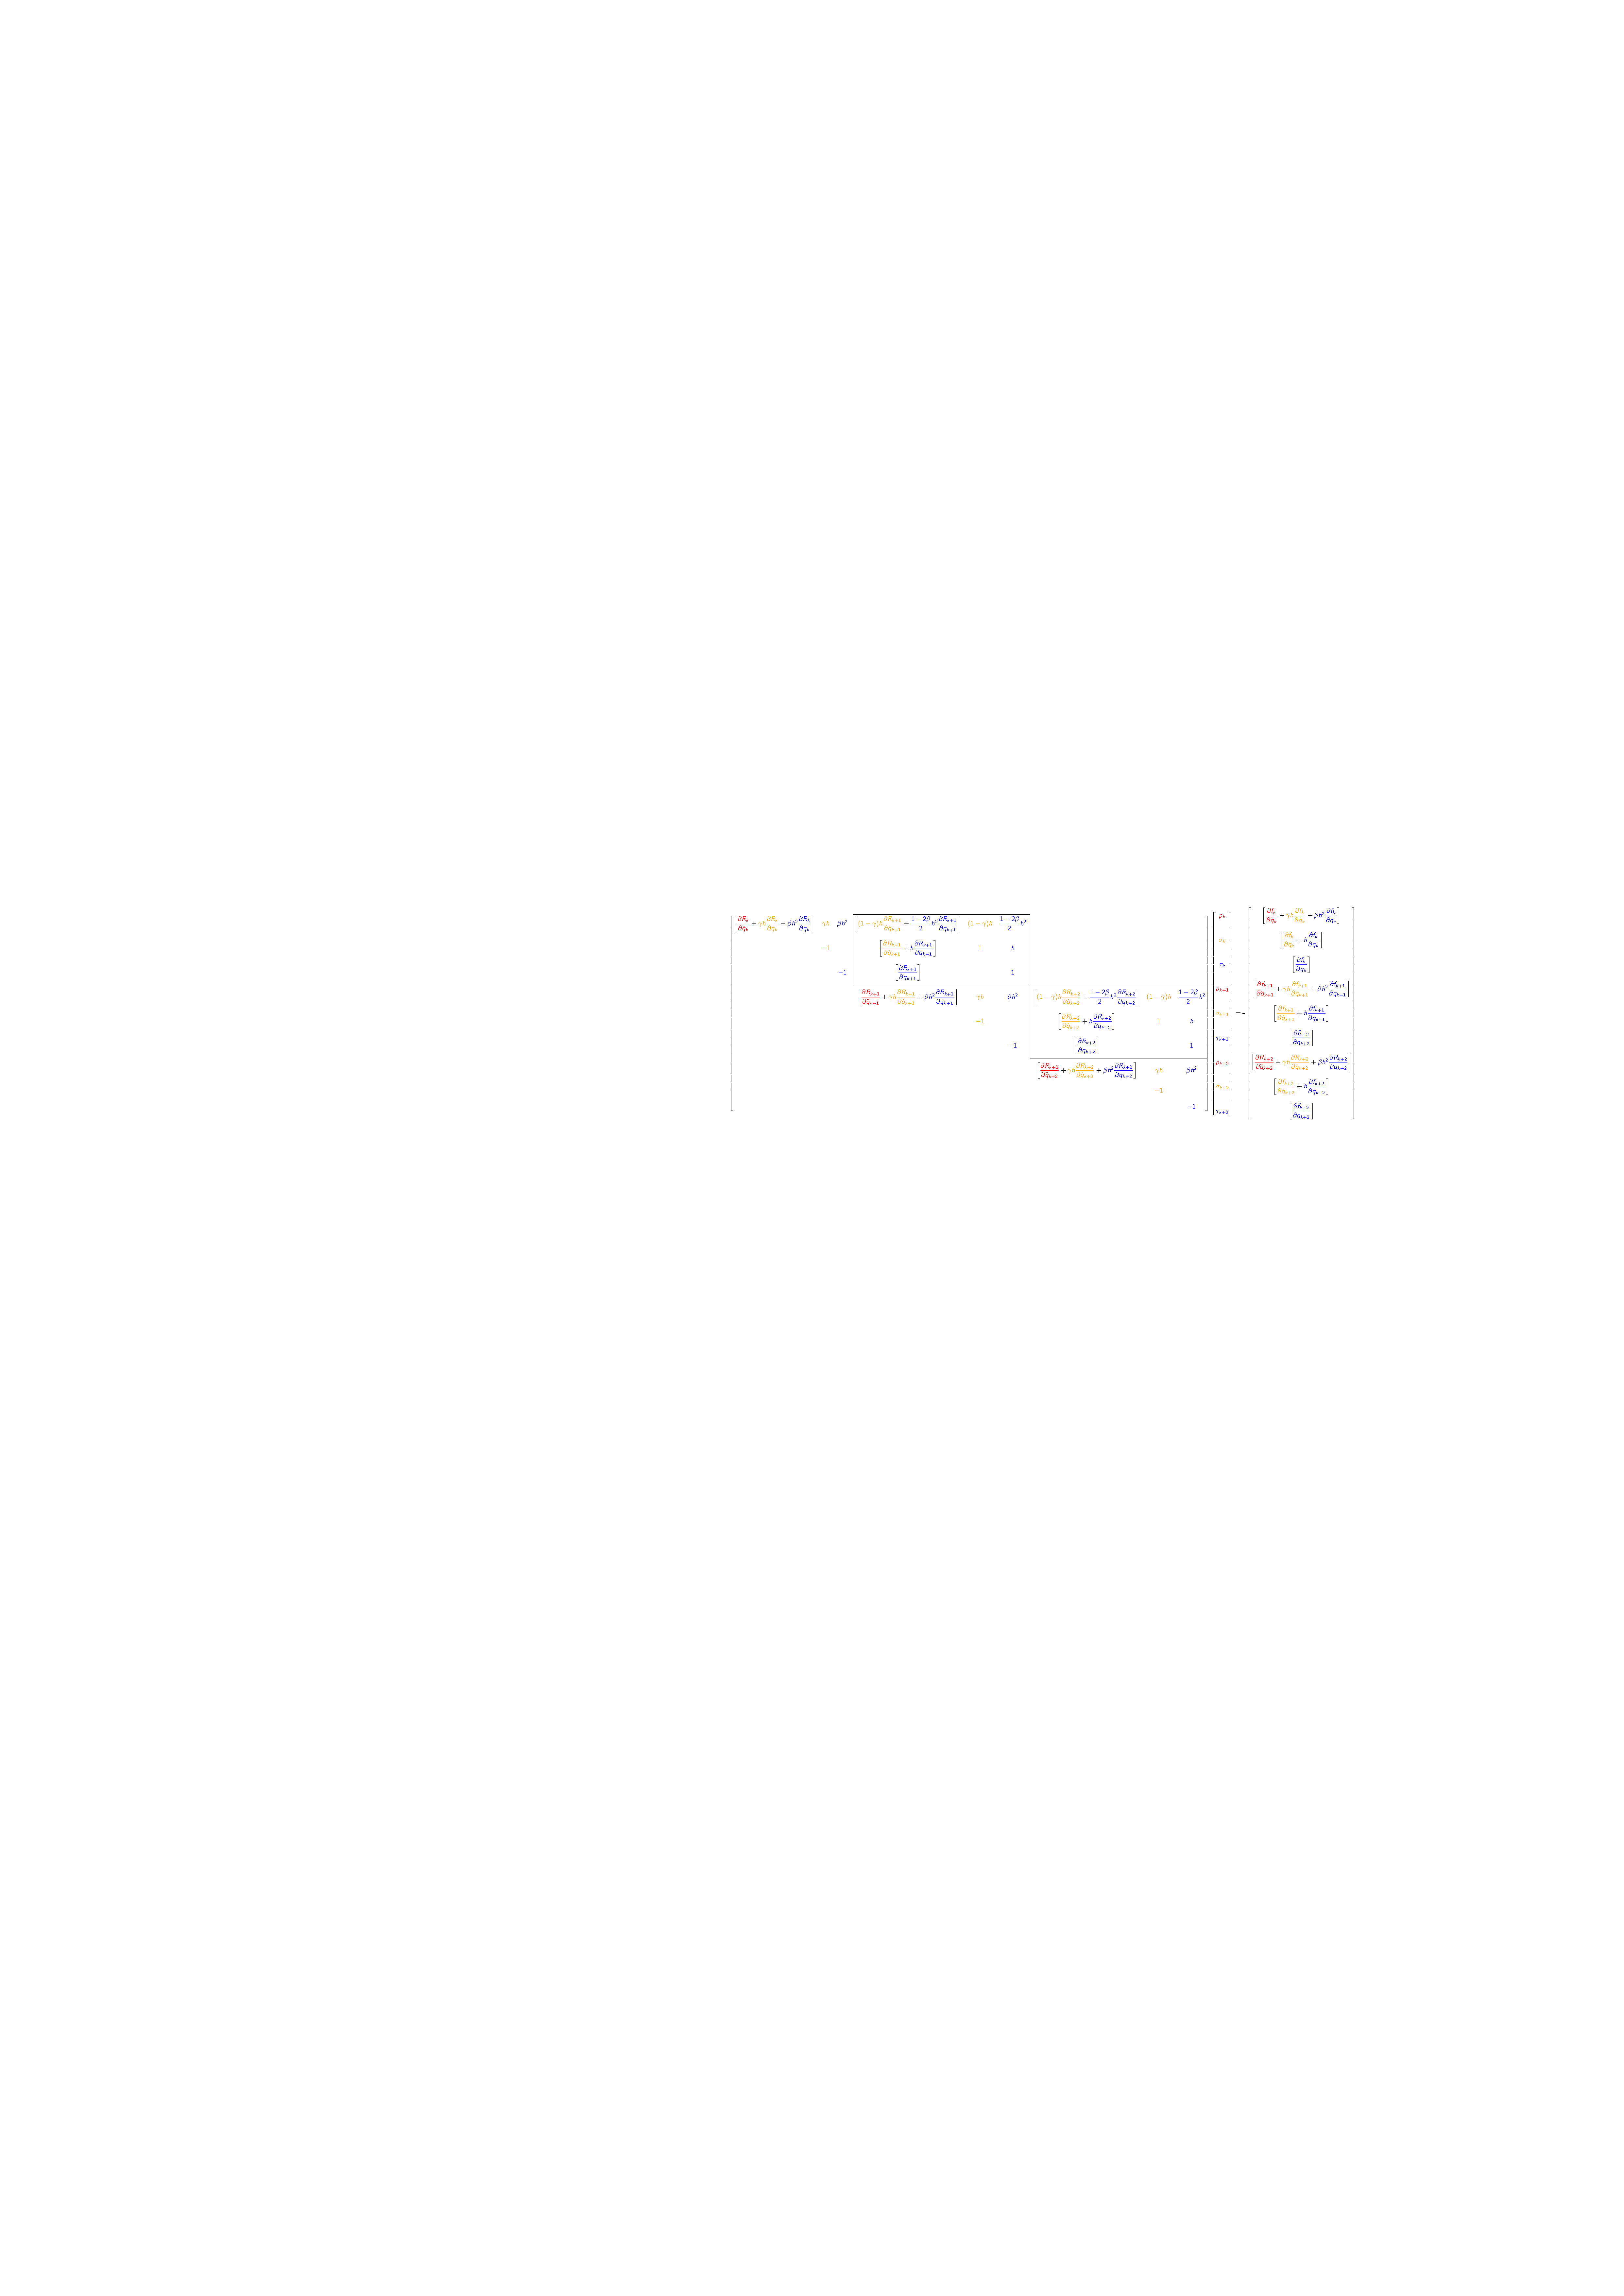
\includegraphics[width=0.925\textwidth]{nbg-reverse-matrix.pdf}
  %        \label{Reverse Mode}
  %      \end{figure}
  %    \end{minipage}

  %    \begin{itemize}

  %    \item Since the equations $S_k$ and $T_k$ are explicit, it becomes
  %      possible to solve \underline{sequentially} for the adjoint
  %      variables at each step. This property is beneficial in terms of
  %      reducing the size of the linear system. The matrix is upper
  %      triangular and we can solve for the adjoint variables sequentially
  %      via back-substitution -- we march backwards in time. The above
  %      treatment is based on the application of chain rule of
  %      differentiation. 

  %   \item Differentiate the terms that carry information within the
  %     current-step from the ones that carry them across time-steps.
  \textbf{Adjoint Equations:}
  The system of equations for the adjoint variables is given by
  $$\textcolor{red}{\pd{\cal{L}}{\ddot{q}_k}},
  \textcolor{orange}{\pd{\cal{L}}{\dot{q}_k}},
  \textcolor{blue}{\pd{\cal{L}}{q_k}} = 0.$$      

  %    \end{itemize}
  \begin{itemize}
  \item Solving for $\phi$ using $\pd{\cal{L}}{{q}_k} = 0$:
    \begin{equation}
      \begin{split}
        \phi_k = \phi_{k+1} + h \left\{ \pd{f_{k+1}}{{q}_{k+1}} \right\}^T + h \left[\pd{R_{k+1}}{{q}_{k+1}} \right]^T \lambda_{k+1}  
      \end{split}
    \end{equation}

  \item Solving for $\psi_k$ using $\pd{\cal{L}}{\dot{q}_k} = 0$:
    \begin{equation}
      \begin{split}
        \psi_k = \psi_{k+1} + h \phi_{k+1}  +h \left\{ \pd{f_{k+1}}{\dot{q}_{k+1}} +  h \pd{f_{k+1}}{{q}_{k+1}} \right\}^T + h\left[ \pd{R_{k+1}}{\dot{q}_{k+1}} +  h \pd{R_{k+1}}{{q}_{k+1}} \right]^T \lambda_{k+1} 
      \end{split}
    \end{equation}

  \item Solving for $\lambda_k$ using $\pd{\cal{L}}{\ddot{q}_k} = 0$:
    
    \begin{equation}
      \begin{split}
        \left[ \pd{R_k}{\ddot{q}_k} + \gamma h \pd{R_k}{\dot{q}_k} + \beta h^2 \pd{R_k}{{q}_k} \right]^T \lambda_k = &- \left\{ \pd{f_k}{\ddot{q}_k} + \gamma h \pd{f_k}{\dot{q}_k} + \beta h^2 \pd{f_k}{{q}_k} \right\}^T \\
        & -  \frac{1}{h}\left\{  \gamma h  \psi_k + \beta h^2   \phi_k \right\}^T\\
        & -  \left\{ (1-\gamma) h \pd{f_{k+1}}{\dot{q}_{k+1}} + \frac{1-2\beta}{2} h^2 \pd{f_{k+1}}{{q}_{k+1}} \right\}^T \\
        & -  \left[ (1-\gamma) h \pd{R_{k+1}}{\dot{q}_{k+1}} + \frac{1-2\beta}{2} h^2 \pd{R_{k+1}}{{q}_{k+1}} \right]^T\lambda_{k+1} \\
        & -  \frac{1}{h} \left\{ (1-\gamma) h \psi_{k+1} + \frac{1-2\beta}{2} h^2 \phi_{k+1} \right\}^T\\
      \end{split}
    \end{equation}
  \end{itemize}
  
  Figure~\ref{fig:nbg-illustration} shows the flow of information across
  states.
  \begin{figure}
    \centering
    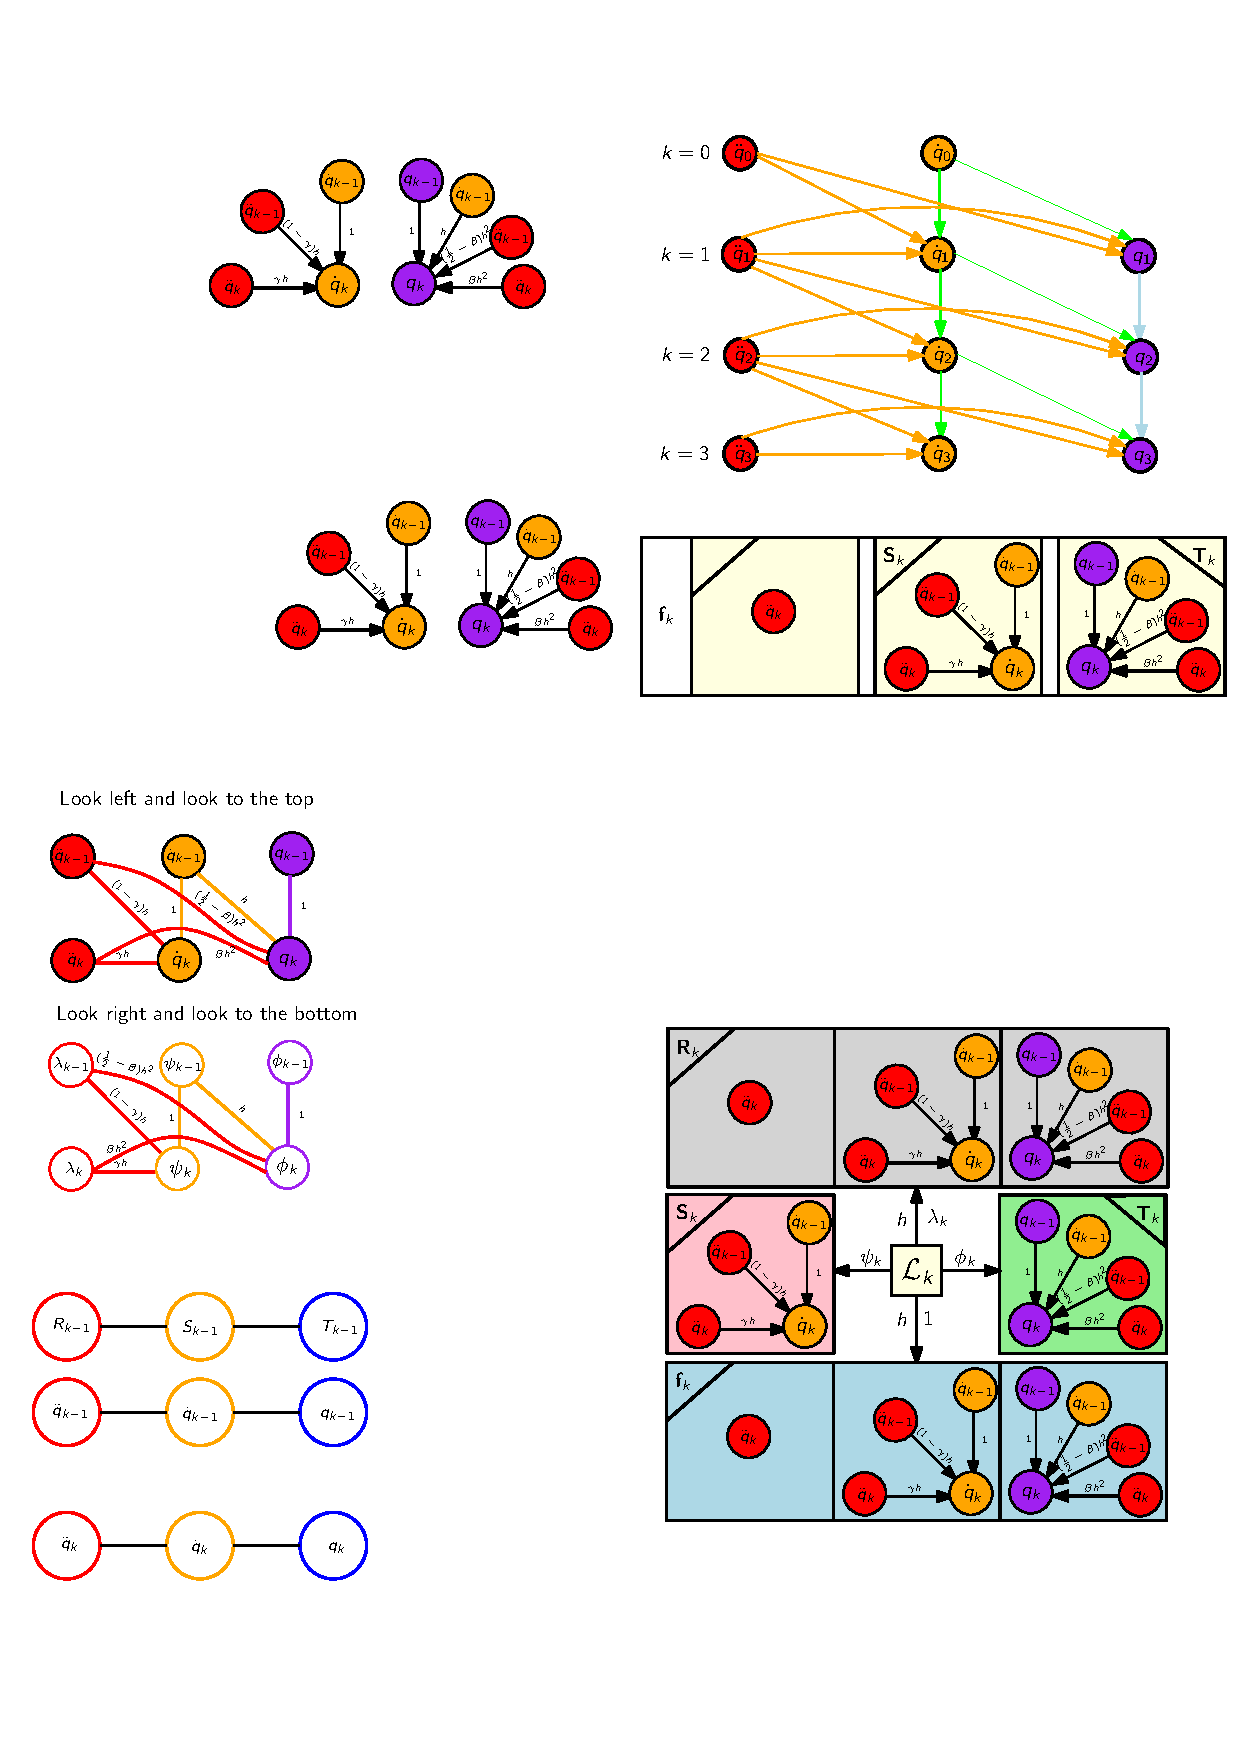
\includegraphics[width=\textwidth]{nbg-chart.pdf}
    %\caption{Illustrations showing the working of NBG method.}
    \label{fig:nbg-illustration}
  \end{figure}
}
\end{frame}
%\end{noheadline}

%         We explore further simplifications by substituting equations.
%
%         \begin{equation}
%           \begin{split}
%             \left[ \frac{1}{h^2} \pd{R_k}{\ddot{q}_k} + \gamma \frac{1}{h} \pd{R_k}{\dot{q}_k} + \beta \pd{R_k}{{q}_k} \right]^T \lambda_k = &- \left\{ \frac{1}{h^2}  \pd{f_k}{\ddot{q}_k} + \gamma \frac{1}{h} \pd{f_k}{\dot{q}_k} + \beta \pd{f_k}{{q}_k} \right\}^T \\
%             & -  \frac{1}{h}\left\{  \gamma \frac{1}{h}  \left( \psi_{k+1} + h \phi_{k+1}  + \left\{ h \pd{f_{k+1}}{\dot{q}_{k+1}} +  h^2 \pd{f_{k+1}}{{q}_{k+1}} \right\}^T + \left[ h \pd{R_{k+1}}{\dot{q}_{k+1}} +  h^2 \pd{R_{k+1}}{{q}_{k+1}} \right]^T \lambda_{k+1}  \right) \right\}^T \\
%             & -  \frac{1}{h}\left\{  \beta  \left( \phi_{k+1} + \left\{h \pd{f_{k+1}}{{q}_{k+1}} \right\}^T + \left[ h \pd{R_{k+1}}{{q}_{k+1}} \right]^T \lambda_{k+1}  \right) \right\}^T\\
%             & -  \left\{ (1-\gamma) \frac{1}{h} \pd{f_{k+1}}{\dot{q}_{k+1}} + \frac{1-2\beta}{2} \pd{f_{k+1}}{{q}_{k+1}} \right\}^T \\
%             & -  \left[ (1-\gamma) \frac{1}{h} \pd{R_{k+1}}{\dot{q}_{k+1}} + \frac{1-2\beta}{2} \pd{R_{k+1}}{{q}_{k+1}} \right]^T\lambda_{k+1} \\
%             & -  \frac{1}{h} \left\{ (1-\gamma) \frac{1}{h} \psi_{k+1} + \frac{1-2\beta}{2} \phi_{k+1} \right\}^T\\
%           \end{split}
%         \end{equation}
%
%         \framebreak


         \framebreak
        
         Grouping the terms together we get:

         \begin{equation}
           \begin{split}
             \left[ \frac{1}{h^2} \pd{R_k}{\ddot{q}_k} + \gamma \frac{1}{h} \pd{R_k}{\dot{q}_k} + \beta \pd{R_k}{{q}_k} \right]^T \lambda_k = &- \left\{ \frac{1}{h^2}  \pd{f_k}{\ddot{q}_k} + \gamma \frac{1}{h} \pd{f_k}{\dot{q}_k} + \beta \pd{f_k}{{q}_k} \right\}^T \\
             & -  \left\{  \gamma \frac{1}{h}  \pd{f_{k+1}}{\dot{q}_{k+1}} +  \gamma \pd{f_{k+1}}{{q}_{k+1}} \right\}^T \\ 
             & -  \left[  \gamma \frac{1}{h}  \pd{R_{k+1}}{\dot{q}_{k+1}} + \gamma \pd{R_{k+1}}{{q}_{k+1}} \right]^T \lambda_{k+1}  \\
             & -  \left\{ \beta \pd{f_{k+1}}{{q}_{k+1}} \right\}^T \\ 
             & - \left[  \beta\pd{R_{k+1}}{{q}_{k+1}} \right]^T \lambda_{k+1}  \\
             & -  \left\{ (1-\gamma) \frac{1}{h} \pd{f_{k+1}}{\dot{q}_{k+1}} + (\frac{1}{2}-\beta) \pd{f_{k+1}}{{q}_{k+1}} \right\}^T \\
             & -  \left[ (1-\gamma) \frac{1}{h} \pd{R_{k+1}}{\dot{q}_{k+1}} + (\frac{1}{2}-\beta) \pd{R_{k+1}}{{q}_{k+1}} \right]^T\lambda_{k+1} \\
             & -  \frac{1}{h} \left\{ \frac{1}{h} \psi_{k+1} + (\frac{1}{2} +\gamma) \phi_{k+1} \right\}^T\\
           \end{split}
         \end{equation}
        
         \begin{equation}
           \begin{split}
             \left[ \frac{1}{h^2} \pd{R_k}{\ddot{q}_k} + \gamma \frac{1}{h} \pd{R_k}{\dot{q}_k} + \beta \pd{R_k}{{q}_k} \right]^T \lambda_k = &- \left\{ \frac{1}{h^2}  \pd{f_k}{\ddot{q}_k} + \gamma \frac{1}{h} \pd{f_k}{\dot{q}_k} + \beta \pd{f_k}{{q}_k} \right\}^T \\
             & -  \left\{  \frac{1}{h} \pd{f_{k+1}}{\dot{q}_{k+1}} +  (\frac{1}{2} +\gamma) \pd{f_{k+1}}{{q}_{k+1}} \right\}^T \\
             & -  \left[  \frac{1}{h} \pd{R_{k+1}}{\dot{q}_{k+1}} +  (\frac{1}{2} +\gamma)  \pd{R_{k+1}}{{q}_{k+1}} \right]^T\lambda_{k+1} \\
             & -  \frac{1}{h} \left\{ \frac{1}{h} \psi_{k+1} + (\frac{1}{2} +\gamma) \phi_{k+1} \right\}^T\\
           \end{split}
         \end{equation}

         Once the primary adjoint variables $\lambda_k$ have been
         determined, the total derivative is readily obtained using
         Eq.\eqref{eqn:nbg-total-derivative}:
         $$\pd{\cal{L}}{x} = \pd{F}{x} = \sum_{k=0}^N h \pd{f_k}{x}^T
         + \sum_{k=0}^N h \pd{R_k}{x}^T \lambda_k.$$ Notice that
         $\pd{S_k}{x} = \pd{T_k}{x} = 0$.  
  


         We can equivalently scale the equation with $1/h^2$ and represent as follows:
         
         \begin{equation}
           \begin{split}
             \left[ \frac{1}{h^2} \pd{R_k}{\ddot{q}_k} + \gamma \frac{1}{h} \pd{R_k}{\dot{q}_k} + \beta \pd{R_k}{{q}_k} \right]^T \lambda_k = &- \left\{ \frac{1}{h^2}  \pd{f_k}{\ddot{q}_k} + \gamma \frac{1}{h} \pd{f_k}{\dot{q}_k} + \beta \pd{f_k}{{q}_k} \right\}^T \\
             & -  \frac{1}{h}\left\{  \gamma \frac{1}{h}  \psi_k + \beta   \phi_k \right\}^T\\
             & -  \left\{ (1-\gamma) \frac{1}{h} \pd{f_{k+1}}{\dot{q}_{k+1}} + \frac{1-2\beta}{2} \pd{f_{k+1}}{{q}_{k+1}} \right\}^T \\
                          & -  \left[ (1-\gamma) \frac{1}{h} \pd{R_{k+1}}{\dot{q}_{k+1}} + \frac{1-2\beta}{2} \pd{R_{k+1}}{{q}_{k+1}} \right]^T\lambda_{k+1} \\
             & -  \frac{1}{h} \left\{ (1-\gamma) \frac{1}{h} \psi_{k+1} + \frac{1-2\beta}{2} \phi_{k+1} \right\}^T\\
           \end{split}
         \end{equation}


         
